\chapter{KLRW Category}

\section{Overview}
\section{Computable Add}


\begin{definition}
 Let $\C$ be a preadditive category. Then the \emph{computable additive completion}
 of $\C$, denoted $\operatorname{CMat}(\C)$, has
 \begin{itemize}
  \item as objects, lists of elements in $\C$.
  \item as morphisms, dependent matrices of morphisms in $\C$.
  Specifically, if $(A_0, A_1, \ldots, A_n), (B_0, B_1, \ldots, B_m) \in \Ob\big(\Mat(\C)\big)$, then
\begin{multline*}
\Hom\big((A_0, A_1, \ldots, A_n), (B_0, B_1, \ldots, B_m)\big) \\
= \left\{
\begin{bmatrix}
  a_{00} & \cdots & a_{0,n-1} \\
  \vdots & \ddots & \vdots \\
  a_{m-1,0} & \cdots & a_{m-1,n-1}
\end{bmatrix}
: a_{ij} \in \Hom(A_j, B_i)
\right\}
\end{multline*}
where $0 \le i \le m-1$ and $0 \le j \le n-1$.

  \item composition is defined by matrix multiplication
  \item identities are given by the identity matrix
  $$ (\idf_{(A_0, \ldots, A_m)})_{i, j} = \begin{cases}
  \idf_{A_i} & \text{reinterpreted as an element of }\Hom(A_i, A_j)
  \text{ by casting along the equality if }i = j
  \\ 0 & \text{ if }i\ne j
  \end{cases}$$.
 \end{itemize}
\end{definition}
  There is a fully faithful functor $G: \C \Rightarrow \CMat(\C)$.

  There is a fully faithful embedding functor $F: \CMat(\C) \Rightarrow \Mat (\C)$.
  It is (nonconstructively) essentially surjective, so $F$ is an equivalence
  of categories.
\begin{definition}
  Given $A = (A_0, \ldots, A_n), B=(B_0, \ldots, B_n)\in \CMat(\C)$, the
  \emph{computable biproduct} of $A$ and $B$ is defined by $A\boxplus_k B = (A_0, \ldots, A_n, B_0, \ldots, B_m)$
\end{definition}
\begin{definition}
  For any $Z\in \CMat (\C)$, the \emph{index type}, denoted $\iota_Z$, is the type
  $\{ 0, \ldots, (\len(Z)-1)\}$, and the indexing function, $X_2: \iota_Z\to \C$,
  is defined by $X_Z(i) = Z_i$.
\end{definition}

\begin{definition}
  Let $n\in \N$. A \emph{positioning} of $1$ black strand with $n$ red strands is
  an element of $\{0, \ldots, n+1\}$. Given positionings of $X$
  and $Y$, the strand set $StrandSpace_{X, Y} = \N$, representing
  the number of dots. (Note here that $\StrandSpace_{X, Y}$ does not depend on
  $X$ or $Y$, but with more black strands it might).
\end{definition}

\begin{definition}
  If $X, Y, Z$ are positionings of $1$ black strand and $n$ red strands
  and $a\in \StrandSpace_{X, Y}$, $b\in \StrandSpace_{Y, Z}$, then their
  composition is given by
  \begin{align*}
    b\circ a &= a + b + \frac{|X-Y| + |Y-Z| - |X-Z|}{2}
    \\ &= a + b + \max (x, y) + \max (y, z) - \max (x, z) - y
  \end{align*}
\end{definition}

\begin{definition}
  Fix a commutative ring $R$. The $\KLRW$ category of $1$ black strand
  and $n$ red strands, denoted $\KLRW$ category of $1$ black strand
  and $n$ red strands, denoted $\KLRW^R_n$, is given by
  \begin{itemize}
    \item $\Ob(\KLRW^R_n)$ is the set of positionings of $1$ black strand
    with $n$ red strands
    \item $\Hom(X, Y)$ is the free $R$-module generated by $\StrandSpace_{X, Y}$.
  \end{itemize}
  Composition in $\KLRW^R_n$ is defined by extending the composition of elements of the strand
  space linearly.

  Since each $\Hom(X, Y)$ is an $R$-module and composition is $R$-linear, $\KLRW^R_n$
  is $R$-linear and thus preadditive.
\end{definition}
\begin{definition}
  Let $\C$ be a preadditive category with a zero object. Then a bounded cochain
  complex of $\C$ is a ($\Z$-graded) cochain complex $A^\bullet$ of $\C$ equipped with a finite set
  $S$ called the support, satisfying
  $\forall i\in \Z, i\in S \Leftrightarrow A^i\not\cong 0$. Note that
  $S$ is uniquely determined by $A^\bullet$, though included
  for computability.
\end{definition}

\section{Bounded Cochain Complexes}
\begin{definition}
  Let $\BK(\C)$ denote the set of bounded cochain complexes in $\C$. THen
  there is a function $F:\BK(\C)\to K^\bullet(\C)$ which forgets the finiteness.
  Then we equip $\BK(\C)$ with the induced category structure of $F$ which makes
  $F$ into a fully faithful functor $F:\BK(\C) \to K^\bullet (\C)$.
\end{definition}

\section{Functor data and functor action}

\subsection{Functor data}
We will now specify the data needed to define how a braiding functor acts. Let $R, S, T \in \mathcal{KLRW}$.

The data of a braiding functor is given by the following functions:
$$
\begin{aligned}
\beta_0 &\colon & \mathcal{KLRW} &\to K^* \\
\beta_1 &\colon & \operatorname{Hom}(R,S) &\to \operatorname{Hom}(\beta_0(R), \beta_0(S)) \\
\beta_2 &\colon & \operatorname{Hom}(R,S) \times \operatorname{Hom}(S,T) &\to \operatorname{Hom}(\beta_0(R), \beta_0(T))
\end{aligned}
$$

In addition to these functions, there must also be proofs that they satisfy $A_\infty$ relations.

Our KLRW category only has composition $\mu_2$, and no higher products. Similarly, the beta-functor has no components higher than $\beta_2$. Therefore the general $[\text{SF}_n]$ axioms for A-infinity functors reduce to a finite list. They are, in particular, the following axioms.

\textbf{[SF\textsubscript{1}].}
For all $f \in \Hom_{\KLRW}(A, B)$,
$$
  \delta_{\beta_0(B)} \circ \beta_1(f) + \beta_1(f) \circ \delta_{\beta_0(A)} = 0.
$$
That is, $\beta_1(f)$ is a chain map from $\beta_0(A)$ to $\beta_0(B)$.

\begin{remark}
  This axiom is automatic from the typing of $\beta_1$: its codomain
  consists of morphisms of cochain complexes, which by definition
  commute with differentials.
\end{remark}

\textbf{[SF\textsubscript{2}].}
For all composable $f \in \Hom_{\KLRW}(A, B)$ and $g \in \Hom_{\KLRW}(B, C)$,
$$
  \beta_1(g \circ f) - \beta_1(g) \circ \beta_1(f)
  = \delta_{\beta_0(C)} \circ \beta_2(f, g) + \beta_2(f, g) \circ \delta_{\beta_0(A)}.
$$
That is, $\beta_1$ is functorial up to the homotopy provided by $\beta_2$.

\begin{remark}
  This is the axiom that gives Maurer--Cartan preservation. If
  $\delta$ is a differential on a complex over $\operatorname{Add}(\KLRW)$
  (i.e.\ $\delta^2 = 0$), then the formula
  $\delta' = \widehat{\beta}_1(\delta) + \widehat{\beta}_2(\delta, \delta)$
  satisfies $(\delta')^2 = 0$, where $\widehat{\beta}_i$ denotes the matrix
  extension.
\end{remark}

\textbf{[SF\textsubscript{3}].}
For all $f \in \Hom_{\KLRW}(A, B)$,
$g \in \Hom_{\KLRW}(B, C)$, and $h \in \Hom_{\KLRW}(C, D)$,
$$
  \beta_2(f, h \circ g) - \beta_2(g \circ f, h)
  = \beta_1(h) \circ \beta_2(f, g) -  \beta_2(g, h)\circ \beta_1(f).
$$
That is, $\beta_2$ satisfies a cocycle condition intertwining source
composition with the target composition mediated by $\beta_1$.

\begin{remark}
  This axiom is needed for iterated cone constructions: when lifting
  a map through a double cone, the correction at the second step must
  be compatible with the correction at the first step.
\end{remark}

\textbf{[SF\textsubscript{4}].}
For all composable $f \in \Hom_{\KLRW}(A, B)$,
$g \in \Hom_{\KLRW}(B, C)$, $h \in \Hom_{\KLRW}(C, D)$, and
$k \in \Hom_{\KLRW}(D, E)$,
$$
  \beta_2(h, k) \circ \beta_2(f, g)= 0.
$$

\begin{remark}
  Since $\beta_2$ produces degree $-1$ maps, their composition has degree
  $-2$. This axiom says this composition vanishes, ensuring no higher
  obstructions arise. For $n \geq 5$, all $[\mathrm{SF}_n]$ axioms are
  automatically satisfied because every term involves either $\beta_k$
  with $k \geq 3$ or $\mu_k$ with $k \geq 3$, both of which are zero.
\end{remark}


One can understand these functions as specifying how the functor acts on the generating elements of our chain complex category. The action of the functor is as follows.

\subsection{Functor action}
\subsubsection{Defining $\beta_0.add$}
Firstly, we may extend the functions acting on $\mathcal{KLRW}$ to act on $\operatorname{Add}(\mathcal{KLRW})$ in a linear sense. We define:
$$\widehat{\beta}_0 \colon \operatorname{Add}(\mathcal{KLRW}) \to K^*$$
by setting:
$$\widehat{\beta}_0\left(\bigoplus_i S_i\right) = \bigoplus_i \beta_0(S_i)$$

\subsubsection{Defining $\beta_1.add$}
Extending the remaining two functions requires more care.

For $\beta_1$, let $\bigoplus_i A_i$ and $\bigoplus_j B_j$ be objects in $\operatorname{Add}(\mathcal{KLRW})$. Let $f \in \operatorname{Hom}\left(\bigoplus_i A_i, \bigoplus_j B_j\right)$. For each pair $k, l$, we project $f$ to its component $f_{k,l} \in \operatorname{Hom}(A_k, B_l)$. We now create $g_{k,l} \in \operatorname{Hom}\left(\widehat{\beta}_0\left(\bigoplus_i A_i\right), \widehat{\beta}_0\left(\bigoplus_j B_j\right)\right)$ by extending this morphism. Formally, $g_{k,l}$ is constructed by composing the canonical projection, the mapped component, and the canonical injection:
$$\widehat{\beta}_0\left(\bigoplus_i A_i\right) \twoheadrightarrow {\beta}_0(A_k) \xrightarrow{\beta_1(f_{k,l})} {\beta}_0(B_l) \hookrightarrow \widehat{\beta}_0\left(\bigoplus_j B_j\right)$$

\subsubsection{Defining $\beta_2.add$}

For $\beta_2$, we construct the extension $\widehat{\beta}_2$ analogously.

\subsubsection{Defining $\beta_0.full$}

\paragraph{Idea}

We now define the action of $\beta$ on a chain complex, i.e. the function

\begin{equation*}
    \beta_0.full: K^*AddKLRW
\rightarrow K^*AddKLRW.
\end{equation*}

The idea is as follows. The definition takes use of chain complexes of block matrices, i.e. elements in $K^*AddAddKLRW$. After constructing an element there, we project into $K^*AddKLRW$.

Let $A^*$ denote the following cochain complex

\[
\cdots \to 0 \to A^{\ell} \xrightarrow{d^{\ell}} A^{\ell+1} \xrightarrow{d^{\ell+1}} \cdots \xrightarrow{d^{r-1}} A^{r} \to 0 \to \cdots
\]

For any $A^i$, consider $B_i ^*:=\beta_0.add(A^i)$ to be the following cochain complex:

\[
\cdots \to 0 \to B^{\ell_i}_{i} \xrightarrow{f_i^{\ell_i}} B^{\ell_i+1}_{i} \xrightarrow{f_i^{\ell_i+1}} \cdots \xrightarrow{f_i^{r_i-1}} B^{r_i}_{i} \to 0 \to \cdots
\]
where the left and right bounds are $l_i$ and $r_i$.

For any $d^i:A^i -> A^{i+1}$, we get $g_i:=\beta_1.add(d^i): B_i ^* \to B_{i+1}^*$. For any two $d^i:A^i -> A^{i+1}, d^{i+1}:A^{i+1} -> A^{i+2}$, we get $h_i:=\beta_2.add(d^i,d^{i+1}): B_i ^* \to B_{i+2}^*[1]$. This gives rise to the following lattice:


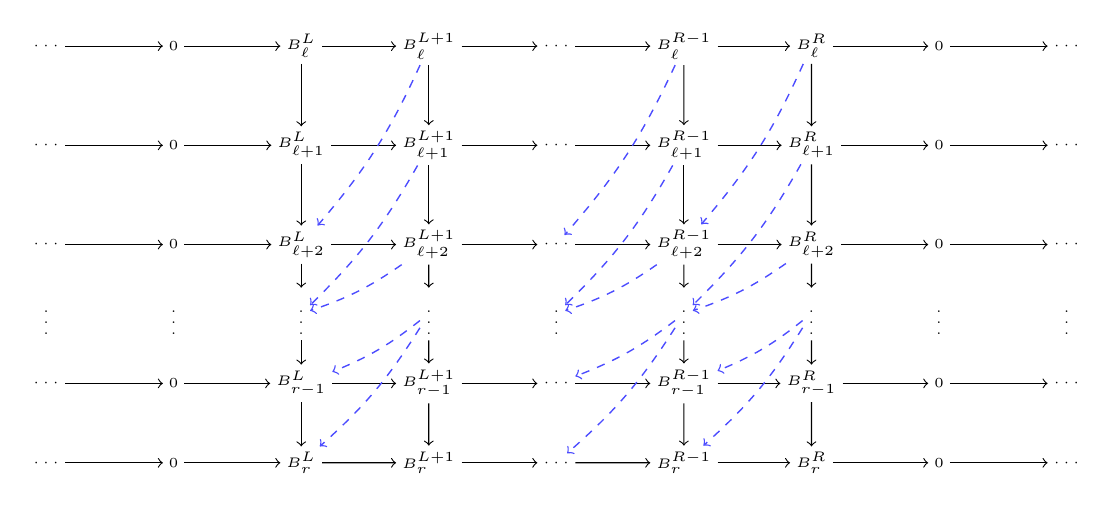
\begin{tikzpicture}[
  scale=0.9,
  every node/.style={
    inner sep=2pt,
    font=\tiny
  }
]
 
% Compact cochain complex style
\def\colspacing{1.8}
\def\rowspacing{1.4}
 
% ==========================================
% ROW 1: i = ℓ (top row)
% ==========================================
\node (A0_m1) at (-\colspacing, 0) {$\cdots$};
\node (A0_0) at (0, 0) {$0$};
\node (A0_1) at (\colspacing, 0) {$B_\ell^L$};
\node (A0_2) at (2*\colspacing, 0) {$B_\ell^{L+1}$};
\node (A0_3) at (3*\colspacing, 0) {$\cdots$};
\node (A0_4) at (4*\colspacing, 0) {$B_\ell^{R-1}$};
\node (A0_5) at (5*\colspacing, 0) {$B_\ell^R$};
\node (A0_6) at (6*\colspacing, 0) {$0$};
\node (A0_7) at (7*\colspacing, 0) {$\cdots$};
 
% ==========================================
% ROW 2: i = ℓ+1
% ==========================================
\node (A1_m1) at (-\colspacing, -\rowspacing) {$\cdots$};
\node (A1_0) at (0, -\rowspacing) {$0$};
\node (A1_1) at (\colspacing, -\rowspacing) {$B_{\ell+1}^L$};
\node (A1_2) at (2*\colspacing, -\rowspacing) {$B_{\ell+1}^{L+1}$};
\node (A1_3) at (3*\colspacing, -\rowspacing) {$\cdots$};
\node (A1_4) at (4*\colspacing, -\rowspacing) {$B_{\ell+1}^{R-1}$};
\node (A1_5) at (5*\colspacing, -\rowspacing) {$B_{\ell+1}^R$};
\node (A1_6) at (6*\colspacing, -\rowspacing) {$0$};
\node (A1_7) at (7*\colspacing, -\rowspacing) {$\cdots$};
 
% ==========================================
% ROW 3: i = ℓ+2
% ==========================================
\node (A2_m1) at (-\colspacing, -2*\rowspacing) {$\cdots$};
\node (A2_0) at (0, -2*\rowspacing) {$0$};
\node (A2_1) at (\colspacing, -2*\rowspacing) {$B_{\ell+2}^L$};
\node (A2_2) at (2*\colspacing, -2*\rowspacing) {$B_{\ell+2}^{L+1}$};
\node (A2_3) at (3*\colspacing, -2*\rowspacing) {$\cdots$};
\node (A2_4) at (4*\colspacing, -2*\rowspacing) {$B_{\ell+2}^{R-1}$};
\node (A2_5) at (5*\colspacing, -2*\rowspacing) {$B_{\ell+2}^R$};
\node (A2_6) at (6*\colspacing, -2*\rowspacing) {$0$};
\node (A2_7) at (7*\colspacing, -2*\rowspacing) {$\cdots$};
 
% ==========================================
% VERTICAL ELLIPSIS ROW (rows ℓ+3 through r-2)
% ==========================================
\node (vdots_m1) at (-\colspacing, -2.7*\rowspacing) {$\vdots$};
\node (vdots_0) at (0, -2.7*\rowspacing) {$\vdots$};
\node (vdots_1) at (\colspacing, -2.7*\rowspacing) {$\vdots$};
\node (vdots_2) at (2*\colspacing, -2.7*\rowspacing) {$\vdots$};
\node (vdots_3) at (3*\colspacing, -2.7*\rowspacing) {$\vdots$};
\node (vdots_4) at (4*\colspacing, -2.7*\rowspacing) {$\vdots$};
\node (vdots_5) at (5*\colspacing, -2.7*\rowspacing) {$\vdots$};
\node (vdots_6) at (6*\colspacing, -2.7*\rowspacing) {$\vdots$};
\node (vdots_7) at (7*\colspacing, -2.7*\rowspacing) {$\vdots$};
 
% ==========================================
% ROW r-1
% ==========================================
\node (A3_m1) at (-\colspacing, -3.4*\rowspacing) {$\cdots$};
\node (A3_0) at (0, -3.4*\rowspacing) {$0$};
\node (A3_1) at (\colspacing, -3.4*\rowspacing) {$B_{r-1}^L$};
\node (A3_2) at (2*\colspacing, -3.4*\rowspacing) {$B_{r-1}^{L+1}$};
\node (A3_3) at (3*\colspacing, -3.4*\rowspacing) {$\cdots$};
\node (A3_4) at (4*\colspacing, -3.4*\rowspacing) {$B_{r-1}^{R-1}$};
\node (A3_5) at (5*\colspacing, -3.4*\rowspacing) {$B_{r-1}^R$};
\node (A3_6) at (6*\colspacing, -3.4*\rowspacing) {$0$};
\node (A3_7) at (7*\colspacing, -3.4*\rowspacing) {$\cdots$};
 
% ==========================================
% ROW r (bottom row)
% ==========================================
\node (A4_m1) at (-\colspacing, -4.2*\rowspacing) {$\cdots$};
\node (A4_0) at (0, -4.2*\rowspacing) {$0$};
\node (A4_1) at (\colspacing, -4.2*\rowspacing) {$B_r^L$};
\node (A4_2) at (2*\colspacing, -4.2*\rowspacing) {$B_r^{L+1}$};
\node (A4_3) at (3*\colspacing, -4.2*\rowspacing) {$\cdots$};
\node (A4_4) at (4*\colspacing, -4.2*\rowspacing) {$B_r^{R-1}$};
\node (A4_5) at (5*\colspacing, -4.2*\rowspacing) {$B_r^R$};
\node (A4_6) at (6*\colspacing, -4.2*\rowspacing) {$0$};
\node (A4_7) at (7*\colspacing, -4.2*\rowspacing) {$\cdots$};
 
% ==========================================
% HORIZONTAL MAPS (along rows) - compact arrows
% ==========================================
 
% Row ℓ
\draw[->] (A0_m1) -- (A0_0);
\draw[->] (A0_0) -- (A0_1);
\draw[->] (A0_1) -- (A0_2);
\draw[->] (A0_2) -- (A0_3);
\draw[->] (A0_3) -- (A0_4);
\draw[->] (A0_4) -- (A0_5);
\draw[->] (A0_5) -- (A0_6);
\draw[->] (A0_6) -- (A0_7);
 
% Row ℓ+1
\draw[->] (A1_m1) -- (A1_0);
\draw[->] (A1_0) -- (A1_1);
\draw[->] (A1_1) -- (A1_2);
\draw[->] (A1_2) -- (A1_3);
\draw[->] (A1_3) -- (A1_4);
\draw[->] (A1_4) -- (A1_5);
\draw[->] (A1_5) -- (A1_6);
\draw[->] (A1_6) -- (A1_7);
 
% Row ℓ+2
\draw[->] (A2_m1) -- (A2_0);
\draw[->] (A2_0) -- (A2_1);
\draw[->] (A2_1) -- (A2_2);
\draw[->] (A2_2) -- (A2_3);
\draw[->] (A2_3) -- (A2_4);
\draw[->] (A2_4) -- (A2_5);
\draw[->] (A2_5) -- (A2_6);
\draw[->] (A2_6) -- (A2_7);
 
% Row r-1
\draw[->] (A3_m1) -- (A3_0);
\draw[->] (A3_0) -- (A3_1);
\draw[->] (A3_1) -- (A3_2);
\draw[->] (A3_2) -- (A3_3);
\draw[->] (A3_3) -- (A3_4);
\draw[->] (A3_4) -- (A3_5);
\draw[->] (A3_5) -- (A3_6);
\draw[->] (A3_6) -- (A3_7);
 
% Row r
\draw[->] (A4_m1) -- (A4_0);
\draw[->] (A4_0) -- (A4_1);
\draw[->] (A4_1) -- (A4_2);
\draw[->] (A4_2) -- (A4_3);
\draw[->] (A4_3) -- (A4_4);
\draw[->] (A4_4) -- (A4_5);
\draw[->] (A4_5) -- (A4_6);
\draw[->] (A4_6) -- (A4_7);
 
% ==========================================
% VERTICAL MAPS (along columns)
% ==========================================
 
% Column L (leftmost)
\draw[->] (A0_1) -- (A1_1);
\draw[->] (A1_1) -- (A2_1);
\draw[->] (A2_1) -- (vdots_1);
\draw[->] (vdots_1) -- (A3_1);
\draw[->] (A3_1) -- (A4_1);
 
% Column L+1
\draw[->] (A0_2) -- (A1_2);
\draw[->] (A1_2) -- (A2_2);
\draw[->] (A2_2) -- (vdots_2);
\draw[->] (vdots_2) -- (A3_2);
\draw[->] (A3_2) -- (A4_2);
 
% Column R-1
\draw[->] (A0_4) -- (A1_4);
\draw[->] (A1_4) -- (A2_4);
\draw[->] (A2_4) -- (vdots_4);
\draw[->] (vdots_4) -- (A3_4);
\draw[->] (A3_4) -- (A4_4);
 
% Column R
\draw[->] (A0_5) -- (A1_5);
\draw[->] (A1_5) -- (A2_5);
\draw[->] (A2_5) -- (vdots_5);
\draw[->] (vdots_5) -- (A3_5);
\draw[->] (A3_5) -- (A4_5);
 
% ==========================================
% DIAGONAL MAPS: B_i^j → B_{i+2}^{j-1}
% From all columns L+1, L+2, ..., R
% Rows ℓ and ℓ+1 map to row ℓ+2
% Row ℓ+2 maps to ellipsis row
% Ellipsis row maps to rows r-1 and r
% ==========================================
 
% From row ℓ:
% A0_2 (L+1) -> A2_1 (L)
\draw[
  ->,
  dashed,
  line width=0.5pt,
  color=blue!70
] (A0_2) to[bend left=8] (A2_1);
 
% A0_4 (R-1) -> A2_3 (R-2, the ellipsis)
\draw[
  ->,
  dashed,
  line width=0.5pt,
  color=blue!70
] (A0_4) to[bend left=8] (A2_3);
 
% A0_5 (R) -> A2_4 (R-1)
\draw[
  ->,
  dashed,
  line width=0.5pt,
  color=blue!70
] (A0_5) to[bend left=8] (A2_4);
 
% From row ℓ+1:
% A1_2 (L+1) -> vdots_1 (L) in ellipsis row
\draw[
  ->,
  dashed,
  line width=0.5pt,
  color=blue!70
] (A1_2) to[bend left=8] (vdots_1);
 
% A1_4 (R-1) -> vdots_3 (R-2)
\draw[
  ->,
  dashed,
  line width=0.5pt,
  color=blue!70
] (A1_4) to[bend left=8] (vdots_3);
 
% A1_5 (R) -> vdots_4 (R-1)
\draw[
  ->,
  dashed,
  line width=0.5pt,
  color=blue!70
] (A1_5) to[bend left=8] (vdots_4);
 
% From row ℓ+2:
% A2_2 (L+1) -> vdots_1 (L) in ellipsis row
\draw[
  ->,
  dashed,
  line width=0.5pt,
  color=blue!70
] (A2_2) to[bend left=8] (vdots_1);
 
% A2_4 (R-1) -> vdots_3 (R-2) in ellipsis row
\draw[
  ->,
  dashed,
  line width=0.5pt,
  color=blue!70
] (A2_4) to[bend left=8] (vdots_3);
 
% A2_5 (R) -> vdots_4 (R-1) in ellipsis row
\draw[
  ->,
  dashed,
  line width=0.5pt,
  color=blue!70
] (A2_5) to[bend left=8] (vdots_4);
 
% From ellipsis row to row r-1:
% vdots_2 (L+1) -> A3_1 (L)
\draw[
  ->,
  dashed,
  line width=0.5pt,
  color=blue!70
] (vdots_2) to[bend left=8] (A3_1);
 
% vdots_4 (R-1) -> A3_3 (R-2, the ellipsis)
\draw[
  ->,
  dashed,
  line width=0.5pt,
  color=blue!70
] (vdots_4) to[bend left=8] (A3_3);
 
% vdots_5 (R) -> A3_4 (R-1)
\draw[
  ->,
  dashed,
  line width=0.5pt,
  color=blue!70
] (vdots_5) to[bend left=8] (A3_4);
 
% From ellipsis row to row r:
% vdots_2 (L+1) -> A4_1 (L)
\draw[
  ->,
  dashed,
  line width=0.5pt,
  color=blue!70
] (vdots_2) to[bend left=8] (A4_1);
 
% vdots_4 (R-1) -> A4_3 (R-2, the ellipsis)
\draw[
  ->,
  dashed,
  line width=0.5pt,
  color=blue!70
] (vdots_4) to[bend left=8] (A4_3);
 
% vdots_5 (R) -> A4_4 (R-1)
\draw[
  ->,
  dashed,
  line width=0.5pt,
  color=blue!70
] (vdots_5) to[bend left=8] (A4_4);
 
\end{tikzpicture}

The cochain complex which we want, is then obtained by taking direct sums along the diagonals. The $A_\infty$-relations ensure that the resulting object is a cochain complex.

\paragraph{Detailed Construction}
Refer to the objects $A^*, B_i^*, g_i, h_i$ as defined above.

Construct first the following object in $K^* AddAddKLRW$.

The objects of the chain complex will be $\mathbb{Z}$-indexed, where each entry is a list of elements in $AddKLRW$. For an index $k$, the element will be the list $\overline{B}^k:=[B_l ^k, B_{l+1}^{k-1},\dots ,B_r ^{k-r+l}]$.

The bounds are as follows. If $L_i$ and $R_i$ is the lower and upper bound of $B_i$, then our lower bound will be $min(L_i-i)$ and the upper bound will be $max(R_i-i)$. The entry will be the $0$-list outside the bounds.

The morphisms will be block matrices, where each entry in the matrix is a morphism between entries in the lists (and thus matrices). For $k$ in these bounds, the morphism $\overline{B}^k\to \overline{B}^{k+1}$ is given by the lower-triangular matrix of the form


\[
\begin{pmatrix}
f & 0 & 0 & 0 & \cdots & 0 \\
g & f & 0 & 0 & \cdots & 0 \\
h & g & f & 0 & \cdots & 0 \\
0 & h & g & f & \cdots & 0 \\
\vdots & \vdots & \vdots & \vdots & \ddots & \vdots \\
0 & 0 & 0 & 0 & \cdots & f
\end{pmatrix}
\]

The $f$'s are the differentials of $B^*_i$, the $g$'s are the chain maps, and the $h$'s are the correction maps. Indices are omitted, but should be possible to infer.

For this to be a differential, it would need to square to 0. This gives rise to the following equations:

\begin{align}
f^2 &= 0 \label{eq:f-squared}\\
fg + gf &= 0 \label{eq:anticomm-fg}\\
fh + g^2 + hf &= 0 \label{eq:cross-term}\\
gh + hg &= 0 \label{eq:anticomm-gh}\\
h^2 &= 0 \label{eq:h-squared}
\end{align}

These can be interpreted as follows:

\begin{itemize}
    \item Equation \ref{eq:f-squared} ensures $f$ is a differential.
    \item Equation \ref{eq:anticomm-fg} ensures $g$ is a chain map: it is $SF_1$ applied to the input differential $d^i$.
    \item Equation \ref{eq:cross-term}, \ref{eq:anticomm-gh} and \ref{eq:h-squared} are the equations corresponding to $SF_2$, $SF_3$ and $SF_4$ respectively, after simplifying with the source differential relation $d^{i+1}d^i=0$.
\end{itemize}




\section{Generating the beta data}
